\documentclass[10pt]{article}
\usepackage[margin=0.75in]{geometry}
\usepackage{amsmath,amssymb}
\usepackage{booktabs}
\usepackage{array}
\usepackage{graphicx}
\usepackage{tabularx}
\usepackage{xurl}
\usepackage{xcolor}
\usepackage{enumitem}
\usepackage{hyperref}
\usepackage{tikz}
\usetikzlibrary{arrows.meta,positioning,shapes.geometric}
\setlength{\emergencystretch}{3em}
\sloppy

\title{Implementation-Pipeline Audit for OccuFly V-JEPA 2.1 Depth and Semantic Scene Completion Experiments}
\author{Pipeline trace generated from local experiment outputs and source code}
\date{July 2, 2026}

\newcommand{\R}{\mathbb{R}}
\newcommand{\B}{B}
\newcommand{\Hin}{H}
\newcommand{\Win}{W}
\newcommand{\Cin}{C}
\newcommand{\Depth}{D}
\newcommand{\Vox}{V}
\newcommand{\stlp}{ST-LP}
\newcommand{\dta}{DTA}
\newcommand{\film}{FiLM}
\newcommand{\dpt}{DPT}
\newcommand{\ssc}{SSC}
\newcommand{\codepath}[1]{\begingroup\small\nolinkurl{#1}\endgroup}

\begin{document}
\maketitle

\section{Scope and Provenance}
This document traces the implementation pipelines that produced the requested result folders and summarizes them in paper-ready architectural language.  The inspected code paths include the supervised depth scripts in \codepath{experiments_related/scripts}, the video-depth projects in \codepath{experiments_related/vjepa21video_scripts}, the CGFormer comparison package, and the V-JEPA 2.1/FoundationSSC semantic scene completion packages in \codepath{experiments_related/scripts_ssc}.  All tensor sizes below refer to the actual OccuFly configuration used in the saved run configurations unless stated otherwise.

\paragraph{Result folders covered.}
\begin{itemize}[leftmargin=*]
  \item Linear depth probes: \codepath{vjepa21_dinov3_linearprobe_occufly_maskaware_rerun_ddp} and \codepath{vjepa21video_features_depth/real_stlp__clip4}.
  \item DPT-FiLM depth probes: \codepath{vjepa21_vitG_dpt_film_occufly_sweep}, \codepath{vjepa21_vitG_final_sfp_dpt_film_occufly_sweep}, \codepath{vjepa21video_features_depth/dptfilm_attention}, and \codepath{30_50train_40_1_4_val_40_5_8_test}.
  \item Semantic scene completion: \codepath{ssc/cgformer_results_comparision}, \codepath{ssc/vjepaF2Dfoundationssc_foundationssc_hybrid_original/...}, \codepath{ssc/vjepaf21oundationssc_mde_warmstart_G}, \codepath{ssc/vjepafoundationssc_foundationssc_hybrid_original_geometry_fix_sm90_corrected_8gpu_20260630_015221}, and \codepath{ssc/vjepafoundationssc_foundationssc_hybrid_original_semantic_reweighting_only_fresh_8gpu_20260701_080802}.
\end{itemize}

\paragraph{Common OccuFly protocol.}
For monocular depth, the standard scene split is train \(\{\texttt{scene\_01},\ldots,\texttt{scene\_05}\}\), validation \(\{\texttt{scene\_06},\texttt{scene\_07}\}\), and test \(\{\texttt{scene\_08},\texttt{scene\_09}\}\), over altitudes \(\{30,40,50\}\) m.  The canonical image resolution is \(384\times384\), patch size is \(16\), V-JEPA 2.1 ViT-Gigantic has \(C=1664\) channels and 48 transformer blocks, and the spatial patch grid is \(24\times24\).  Depth is metric and clipped/evaluated in \([0.001,80]\) m.  Invalid depth pixels are finite-masked before resizing; loss and metrics use only valid pixels.

\section{Frozen V-JEPA 2.1/DINOv3 Mask-Aware Linear Depth Probe}
\subsection{High-Level Overview}
This pipeline is a strict frozen-backbone linear probe for monocular metric depth.  RGB images are encoded by a frozen V-JEPA 2.1 ViT-Gigantic backbone, the final dense patch map is passed to a DINOv3-style \(\texttt{SyncBatchNorm}+\texttt{Conv2d}(1\times1)\) linear head, and the 256-channel output is converted to metric depth by \texttt{FeaturesToDepth}.  The result folder \codepath{vjepa21_dinov3_linearprobe_occufly_maskaware_rerun_ddp} was trained with distributed data parallelism, global batch size 8, 20 epochs, and LR/WD sweeps.  The inspected completed point \codepath{lr_1p5e_3__wd_1e_3} uses \(14{,}804\) training samples, \(1{,}965\) validation samples, and \(3{,}842\) test samples.

\paragraph{Implementation paths.}
The core implementation is \codepath{experiments_related/scripts/06_vjepa21_dinov3_linearprobe_occufly.py}.  The DDP sweep/resume launcher is \codepath{experiments_related/scripts/linearprobe/run_maskaware_occufly_ddp_sweep_resume.sh}, and the altitude/BatchNorm probe variants are documented and launched from \codepath{experiments_related/scripts/linearprobe/README.md} and related \codepath{experiments_related/scripts/linearprobe/train_occufly_dino_linear_bn_*.py} scripts.  The V-JEPA 2.1/DINO bridge used by this family is \codepath{experiments_related/scripts/vjepa21_dinov3_depth_adapter.py}.

\begin{center}
\resizebox{\linewidth}{!}{%
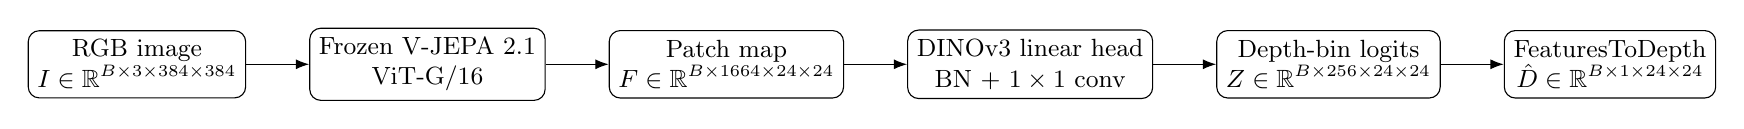
\begin{tikzpicture}[node distance=8mm, every node/.style={draw, rounded corners, align=center, font=\small, minimum height=7mm}, >=Latex]
\node (rgb) {RGB image\\\(I\in\R^{B\times3\times384\times384}\)};
\node[right=of rgb] (vj) {Frozen V-JEPA 2.1\\ViT-G/16};
\node[right=of vj] (feat) {Patch map\\\(F\in\R^{B\times1664\times24\times24}\)};
\node[right=of feat] (head) {DINOv3 linear head\\BN + \(1\times1\) conv};
\node[right=of head] (logits) {Depth-bin logits\\\(Z\in\R^{B\times256\times24\times24}\)};
\node[right=of logits] (depth) {FeaturesToDepth\\\(\hat{D}\in\R^{B\times1\times24\times24}\)};
\draw[->] (rgb) -- (vj);
\draw[->] (vj) -- (feat);
\draw[->] (feat) -- (head);
\draw[->] (head) -- (logits);
\draw[->] (logits) -- (depth);
\end{tikzpicture}
}
\end{center}

\subsection{Mathematical Formulation}
Let \(I_b\in\R^{3\times384\times384}\).  The frozen encoder \(E_{\theta}^{\mathrm{VJ}}\) returns a patch feature tensor
\[
F_b = E_{\theta}^{\mathrm{VJ}}(I_b)\in\R^{1664\times24\times24}, \qquad \theta \text{ frozen}.
\]
The probe is a per-location affine classifier over depth bins:
\[
Z_b(:,u,v)=W\,\mathrm{BN}(F_b(:,u,v))+a,\qquad W\in\R^{256\times1664}.
\]
For linear-bin conversion, with \(d_k\) uniformly spaced in \([d_{\min},d_{\max}]\), \texttt{FeaturesToDepth} computes normalized nonnegative bin weights \(p_{k,u,v}\) and
\[
\hat{D}_{b,u,v}=\sum_{k=1}^{256}p_{b,k,u,v}d_k.
\]
The ground-truth depth \(D\) and validity mask \(M\) are resized using weighted mask-aware interpolation:
\[
D'=\frac{\mathrm{resize}(D\odot M)}{\max(\mathrm{resize}(M),\epsilon)},\qquad
M'=\mathrm{resize}(M)>\tau .
\]
The training criterion is masked scale-invariant depth loss (\texttt{SIGLOSS}) and metrics include RMSE, AbsRel, and log-RMSE over \(M'\).

\section{V-JEPA 2.1 Video Spatio-Temporal Linear Probe (\stlp)}
\subsection{Definition of ST-LP}
\textbf{\stlp} means \textbf{Spatio-Temporal Linear Probe}.  It is the video-mode analogue of the image linear depth probe, but it preserves the V-JEPA 2.1 video tubelet axis instead of averaging it.  The folder \codepath{vjepa21video_features_depth/real_stlp__clip4} uses target-centered real clips with four RGB frames.  The backbone is frozen, selected layer is the final V-JEPA 2.1 layer \(47\), and the saved run reports 858,880 trainable decoder parameters.

\paragraph{Implementation paths.}
The video ST-LP project lives under \codepath{experiments_related/vjepa21video_scripts}.  The main trainer is \codepath{experiments_related/vjepa21video_scripts/scripts/train_stlp_depth.py}; the sequential ablation runner is \codepath{experiments_related/vjepa21video_scripts/scripts/run_all_stlp_experiments.py}; and the implementation modules are \codepath{experiments_related/vjepa21video_scripts/src/vjepa21video_depth/depth_heads.py}, \codepath{experiments_related/vjepa21video_scripts/src/vjepa21video_depth/vjepa_backbone.py}, \codepath{experiments_related/vjepa21video_scripts/src/vjepa21video_depth/occufly_data.py}, and \codepath{experiments_related/vjepa21video_scripts/src/vjepa21video_depth/losses_metrics.py}.

\begin{center}
\resizebox{\linewidth}{!}{%
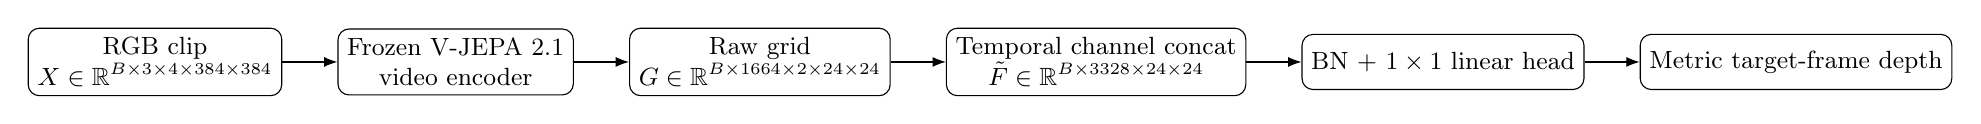
\begin{tikzpicture}[node distance=7mm, every node/.style={draw, rounded corners, align=center, font=\small, minimum height=7mm}, >=Latex]
\node (clip) {RGB clip\\\(X\in\R^{B\times3\times4\times384\times384}\)};
\node[right=of clip] (enc) {Frozen V-JEPA 2.1\\video encoder};
\node[right=of enc] (grid) {Raw grid\\\(G\in\R^{B\times1664\times2\times24\times24}\)};
\node[right=of grid] (concat) {Temporal channel concat\\\(\tilde{F}\in\R^{B\times3328\times24\times24}\)};
\node[right=of concat] (lin) {BN + \(1\times1\) linear head};
\node[right=of lin] (out) {Metric target-frame depth};
\draw[->] (clip) -- (enc);
\draw[->] (enc) -- (grid);
\draw[->] (grid) -- (concat);
\draw[->] (concat) -- (lin);
\draw[->] (lin) -- (out);
\end{tikzpicture}
}
\end{center}

\subsection{Inputs, Outputs, and Ablation Meaning}
For a 4-frame clip and V-JEPA 2.1 tubelet size 2, \(T'=4/2=2\).  The encoder output is
\[
G=E_{\theta}^{\mathrm{video}}(X)\in\R^{B\times C\times T'\times H'\times W'}
=\R^{B\times1664\times2\times24\times24}.
\]
\stlp{} reorders the tensor by
\[
\tilde{F}_{b,(tC+c),u,v}=G_{b,c,t,u,v},\quad
\tilde{F}\in\R^{B\times(T'C)\times H'\times W'}=\R^{B\times3328\times24\times24}.
\]
The linear head weight tensor is \(W\in\R^{256\times3328\times1\times1}\), and temporal importance can be recovered by reshaping \(W\rightarrow\R^{256\times T'\times C}\) and summing absolute mass per tubelet.  The three intended video ablations are: \codepath{repeated_stlp}, where the same target frame is repeated; \codepath{real_stlp}, where the target-centered temporal context is real; and \codepath{shuffled_stlp}, where real context frames are deterministically shuffled.  Missing target depth and first/last frames are excluded from training and evaluation.

\section{Image-Mode V-JEPA 2.1 DPT-FiLM Depth Decoder}
\subsection{High-Level Overview}
The DPT-FiLM pipeline replaces the linear head with a multi-layer DPT decoder and metadata conditioning.  The folder \codepath{vjepa21_vitG_dpt_film_occufly_sweep} uses selected V-JEPA 2.1 transformer layers \(\{11,23,37,47\}\), each reshaped to a \(24\times24\) patch map, then passed through DINOv3 DPT reassembly/projection, FiLM metadata modulation, DPT fusion/refinement, and depth-bin conversion.

\paragraph{Implementation paths.}
The image-mode DPT-FiLM trainer is \codepath{experiments_related/scripts/dpt_decoder/train_vjepa21_vitG_dpt_film_occufly.py}.  Its run notes and command templates are in \codepath{experiments_related/scripts/dpt_decoder/README.md}.  The implementation reuses the DINOv3 depth-head adapter and V-JEPA 2.1 checkpoint loading utilities from \codepath{experiments_related/scripts/vjepa21_dinov3_depth_adapter.py}.

\textbf{FiLM} is \textbf{Feature-wise Linear Modulation}.  The metadata vector is
\[
m=[h_{\mathrm{norm}}, f_x/W, f_y/H, c_x/W-0.5, c_y/H-0.5]\in\R^5,\qquad
h_{\mathrm{norm}}=(h-40)/10 .
\]
A metadata MLP maps \(m\) to \(e_m\in\R^{128}\).  Each DPT level \(l\) applies
\[
\mathrm{FiLM}_l(F_l,e_m)=F_l\odot\left(1+\gamma_l(e_m)\right)+\beta_l(e_m),
\]
where \(\gamma_l,\beta_l\in\R^{C_d}\) are predicted by a linear layer initialized to identity behavior.  In the inspected run configs, \(C_d=256\), hidden channels are 32, and DPT post-process channels are \([128,256,512,1024]\).

\begin{center}
\resizebox{\linewidth}{!}{%
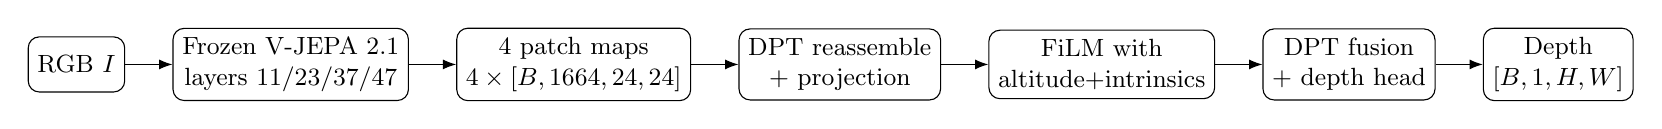
\begin{tikzpicture}[node distance=6mm, every node/.style={draw, rounded corners, align=center, font=\small, minimum height=7mm}, >=Latex]
\node (rgb) {RGB \(I\)};
\node[right=of rgb] (vj) {Frozen V-JEPA 2.1\\layers 11/23/37/47};
\node[right=of vj] (maps) {4 patch maps\\\(4\times[B,1664,24,24]\)};
\node[right=of maps] (dpt) {DPT reassemble\\+ projection};
\node[right=of dpt] (film) {FiLM with\\altitude+intrinsics};
\node[right=of film] (fusion) {DPT fusion\\+ depth head};
\node[right=of fusion] (depth) {Depth\\\([B,1,H,W]\)};
\draw[->] (rgb) -- (vj);
\draw[->] (vj) -- (maps);
\draw[->] (maps) -- (dpt);
\draw[->] (dpt) -- (film);
\draw[->] (film) -- (fusion);
\draw[->] (fusion) -- (depth);
\end{tikzpicture}
}
\end{center}

\subsection{Final-Layer SFP DPT-FiLM Variant}
The folder \codepath{vjepa21_vitG_final_sfp_dpt_film_occufly_sweep} uses the same depth target and FiLM conditioning but changes the feature source.  Instead of requesting four intermediate transformer layers, it takes the final V-JEPA 2.1 token sequence only, reshapes it to \(F^{47}\in\R^{B\times1664\times24\times24}\), and expands it with a local \textbf{SFP} (\textbf{Simple Feature Pyramid}) adapted from ViTDet/Detectron2:
\[
\mathrm{SFP}(F^{47})=\{F_4,F_2,F_1,F_{1/2}\},\quad
F_s\in\R^{B\times256\times(24s)\times(24s)},\quad s\in\{4,2,1,1/2\}.
\]
Thus the four DPT levels are approximately \(96\times96\), \(48\times48\), \(24\times24\), and \(12\times12\), each with 256 channels.  The DPT post-process channels in this variant are \([256,256,256,256]\), and the run uses frozen V-JEPA 2.1, distributed training, 5 GPUs for the inspected point, and the same metric-depth conversion.

\paragraph{Implementation paths.}
The final-layer SFP variant is implemented in \codepath{experiments_related/scripts/dpt_decoder/train_vjepa21_vitG_final_sfp_dpt_film_occufly.py}.  The same README, \codepath{experiments_related/scripts/dpt_decoder/README.md}, records the intended command line and explicitly distinguishes this final-token SFP path from the four-intermediate-layer DPT-FiLM path.

\section{Video DPT-FiLM with Dense Temporal Attention (\dta)}
\subsection{High-Level Overview}
The folder \codepath{vjepa21video_features_depth/dptfilm_attention} implements video-mode DPT-FiLM.  Its \codepath{real_dta__clip4/lr_1e_-3__wd_1e_-3} run uses four-frame clips, selected layers \(\{11,23,37,47\}\), frozen V-JEPA 2.1-Gigantic, 30 epochs, \(\mathrm{lr}=10^{-3}\), \(\mathrm{wd}=10^{-3}\), metadata dimension 128, and 8 temporal attention heads.  \textbf{\dta} means \textbf{Dense Temporal Attention}: at each spatial cell and selected layer, a learned query attends over the tubelet features.

\paragraph{Implementation paths.}
The video DPT-FiLM+DTA project lives at \codepath{experiments_related/vjepa21video_scripts/vjepa21video_dptfilm_attention}.  The main trainer is \codepath{experiments_related/vjepa21video_scripts/vjepa21video_dptfilm_attention/scripts/train_video_dptfilm_attention.py}; the sequential runner is \codepath{experiments_related/vjepa21video_scripts/vjepa21video_dptfilm_attention/scripts/run_all_dptfilm_attention_experiments.py}; and the relevant model modules are \codepath{experiments_related/vjepa21video_scripts/vjepa21video_dptfilm_attention/src/vjepa21video_dptfilm_attention/model.py}, \codepath{experiments_related/vjepa21video_scripts/vjepa21video_dptfilm_attention/src/vjepa21video_dptfilm_attention/temporal_attention.py}, \codepath{experiments_related/vjepa21video_scripts/vjepa21video_dptfilm_attention/src/vjepa21video_dptfilm_attention/dpt_film.py}, and \codepath{experiments_related/vjepa21video_scripts/vjepa21video_dptfilm_attention/src/vjepa21video_dptfilm_attention/vjepa21_video_adapter.py}.

\begin{center}
\resizebox{\linewidth}{!}{%
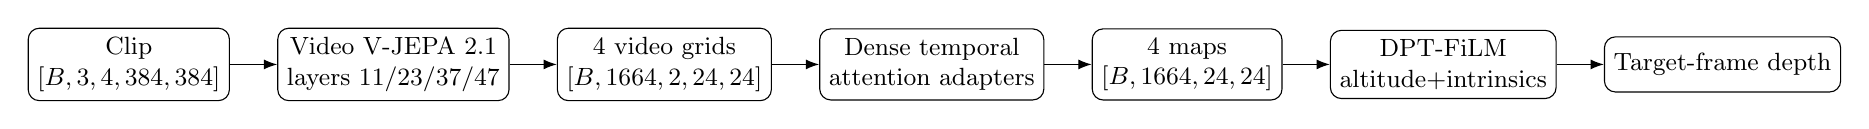
\begin{tikzpicture}[node distance=6mm, every node/.style={draw, rounded corners, align=center, font=\small, minimum height=7mm}, >=Latex]
\node (clip) {Clip\\\([B,3,4,384,384]\)};
\node[right=of clip] (vj) {Video V-JEPA 2.1\\layers 11/23/37/47};
\node[right=of vj] (grids) {4 video grids\\\([B,1664,2,24,24]\)};
\node[right=of grids] (dta) {Dense temporal\\attention adapters};
\node[right=of dta] (maps) {4 maps\\\([B,1664,24,24]\)};
\node[right=of maps] (dpt) {DPT-FiLM\\altitude+intrinsics};
\node[right=of dpt] (depth) {Target-frame depth};
\draw[->] (clip) -- (vj);
\draw[->] (vj) -- (grids);
\draw[->] (grids) -- (dta);
\draw[->] (dta) -- (maps);
\draw[->] (maps) -- (dpt);
\draw[->] (dpt) -- (depth);
\end{tikzpicture}
}
\end{center}

\subsection{Dense Temporal Attention Notation}
For each selected layer \(l\), the video backbone returns \(G_l\in\R^{B\times1664\times T'\times24\times24}\), with \(T'=2\) for 4-frame clips and \(T'=4\) for 8-frame clips.  At every spatial site \((u,v)\), the adapter forms a temporal token sequence
\[
S_{b,u,v}^{(l)} = [G_{b,:,1,u,v}^{(l)},\ldots,G_{b,:,T',u,v}^{(l)}]\in\R^{T'\times1664}.
\]
A \(1\times1\times1\) projection reduces channels to \(A=512\), a learned query \(q\in\R^{1\times A}\) attends over the \(T'\) tokens with 8-head multi-head attention, and a residual interpolation with initial scale \(0.1\) yields
\[
\bar{F}_{b,:,u,v}^{(l)}
= \mathrm{mean}_t(G_{b,:,t,u,v}^{(l)})+
\alpha\left(\mathrm{Expand}(\mathrm{MHA}(q,K,V))-\mathrm{mean}_t(G_{b,:,t,u,v}^{(l)})\right).
\]
The adapted maps \(\{\bar{F}^{(l)}\}\) are consumed by the same DPT-FiLM decoder as the image-mode four-layer variant.  The available tags are \codepath{repeated_dta}, \codepath{real_dta}, and \codepath{shuffled_dta}.

\section{Altitude-Split DPT-FiLM Depth Protocol}
The folder \codepath{30_50train_40_1_4_val_40_5_8_test} uses the same DPT-FiLM training code path but a different generalization protocol: train on 30 m and 50 m data, validate on 40 m scenes 01--04, and test on 40 m scenes 05--08.  This is not merely a random scene split; it explicitly tests whether the learned depth model interpolates to the unseen middle altitude.  The saved sweep contains LR/WD points and per-altitude metrics.  In notation, the training set is
\[
\mathcal{D}_{\mathrm{train}}=\{(I,D,m): h\in\{30,50\}\},\quad
\mathcal{D}_{\mathrm{val/test}}\subset\{(I,D,m): h=40\},
\]
with the same metadata definition \(m=[h_{\mathrm{norm}}, f_x/W, f_y/H, c_x/W-0.5, c_y/H-0.5]\).  This folder should be reported as an altitude-interpolation stress test for the DPT-FiLM depth decoder.

\paragraph{Implementation paths.}
This split is controlled by the split-protocol support in \codepath{experiments_related/scripts/dpt_decoder/train_vjepa21_vitG_dpt_film_occufly.py}.  The launcher/logs in the output folder point back to that trainer with a non-default split protocol that trains on altitudes 30 and 50, validates on 40 m scenes 01--04, and tests on 40 m scenes 05--08.

\section{CGFormer-Based Semantic Scene Completion Comparison}
\subsection{High-Level Overview}
The folder \codepath{ssc/cgformer_results_comparision} is an aggregate comparison of six CGFormer/OccuFly SSC runs: \codepath{dav2prior}, \codepath{m2_vjepa_distill_projector_current}, \codepath{m3_latent_view}, \codepath{m4_masked3d_projector_current}, and two V-JEPA 2.1 ViT-G DPT-FiLM depth-prior runs.  It is a reporting layer, not a new model: \codepath{runs_wide.csv}, \codepath{metrics_long.csv}, \codepath{leaderboard_long.csv}, \codepath{altitude_metrics_long.csv}, and \codepath{class_metrics_long.csv} are generated from each run's \codepath{results_ssc.csv} and \codepath{metrics_test.json}.

\paragraph{Implementation paths.}
The comparison dashboard and table generator in the result folder are \codepath{experiments_related/outputs/results/ssc/cgformer_results_comparision/view_results.py} and \codepath{experiments_related/outputs/results/ssc/cgformer_results_comparision/README.md}.  The CGFormer OccuFly preparation/evaluation utilities are under \codepath{experiments_related/scripts_ssc/cgformer/common}, with V-JEPA 2.1/DPT-FiLM prior export and launch scripts under \codepath{experiments_related/scripts_ssc/cgformer/vitGFilmaltitudeconditioning}.  The local baseline model repository is \codepath{CGFormer}.

CGFormer is used as a semantic scene completion baseline family with image-to-BEV/voxel modules from the local \texttt{CGFormer} codebase.  The comparison emphasizes occupied-class mIoU, occupied IoU, class-wise IoU, altitude-stratified metrics, and deltas against the DAV2-prior baseline.  DAV2 means Depth Anything V2; V-JEPA 2.1 means Video Joint Embedding Predictive Architecture; BEV means Bird's-Eye View; SSC means Semantic Scene Completion.

\section{V-JEPA 2.1/F2D + FoundationSSC Hybrid SSC}
\subsection{Architecture Overview}
The requested \codepath{vjepaF2Dfoundationssc_foundationssc_hybrid_original} and corrected \codepath{vjepafoundationssc_...} folders implement a hybrid semantic scene completion system.  The front end is V-JEPA 2.1 plus DPT-FiLM depth/probability estimation; the 3D back end is real FoundationSSC/MMCV/MMDetection/DFA3D with OccuFly geometry patched into its config before module construction.

\paragraph{Implementation paths.}
The active corrected FoundationSSC hybrid source is \codepath{experiments_related/scripts_ssc/vjepafoundationssc_foundationssc_hybrid_original}.  The main trainer is \codepath{experiments_related/scripts_ssc/vjepafoundationssc_foundationssc_hybrid_original/vjepafoundationssc/train_vjepa_occufly_ssc.py}; the depth front end is \codepath{experiments_related/scripts_ssc/vjepafoundationssc_foundationssc_hybrid_original/vjepafoundationssc/dpt_film_depth_probability_head.py}; the V-JEPA 2.1 backbone wrapper is \codepath{experiments_related/scripts_ssc/vjepafoundationssc_foundationssc_hybrid_original/vjepafoundationssc/backbone_factory.py}; the lifting code is \codepath{experiments_related/scripts_ssc/vjepafoundationssc_foundationssc_hybrid_original/vjepafoundationssc/frustum_voxel_pool.py}; losses and metrics are \codepath{experiments_related/scripts_ssc/vjepafoundationssc_foundationssc_hybrid_original/vjepafoundationssc/losses_ssc.py} and \codepath{experiments_related/scripts_ssc/vjepafoundationssc_foundationssc_hybrid_original/vjepafoundationssc/metrics_ssc.py}; and the real FoundationSSC adapters are in \codepath{experiments_related/scripts_ssc/vjepafoundationssc_foundationssc_hybrid_original/vjepafoundationssc/foundation_ssc/real_adapters.py}.  The older F2D package variant is under \codepath{experiments_related/scripts_ssc/vjepaF2Dfoundationssc_foundationssc_hybrid_original}.

\begin{center}
\resizebox{\linewidth}{!}{%
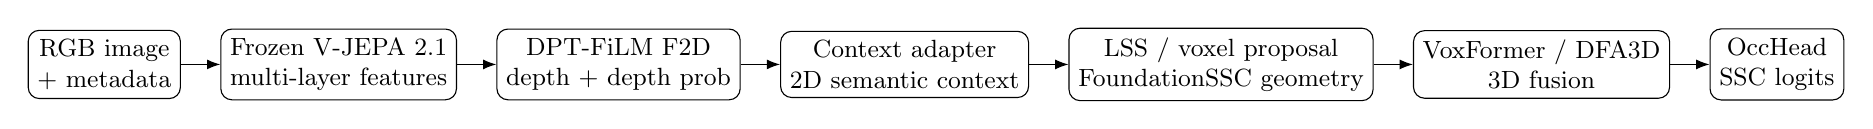
\begin{tikzpicture}[node distance=5mm, every node/.style={draw, rounded corners, align=center, font=\small, minimum height=7mm}, >=Latex]
\node (rgb) {RGB image\\+ metadata};
\node[right=of rgb] (vj) {Frozen V-JEPA 2.1\\multi-layer features};
\node[right=of vj] (dpt) {DPT-FiLM F2D\\depth + depth prob};
\node[right=of dpt] (ctx) {Context adapter\\2D semantic context};
\node[right=of ctx] (lss) {LSS / voxel proposal\\FoundationSSC geometry};
\node[right=of lss] (vox) {VoxFormer / DFA3D\\3D fusion};
\node[right=of vox] (head) {OccHead\\SSC logits};
\draw[->] (rgb) -- (vj);
\draw[->] (vj) -- (dpt);
\draw[->] (dpt) -- (ctx);
\draw[->] (ctx) -- (lss);
\draw[->] (lss) -- (vox);
\draw[->] (vox) -- (head);
\end{tikzpicture}
}
\end{center}

\textbf{F2D} is used here as \textbf{features-to-depth}: DPT-FiLM predicts both dense metric depth \(\hat{D}\) and a depth-bin probability tensor \(P_D\).  \textbf{LSS} is \textbf{Lift-Splat-Shoot}; this is the camera-to-voxel lifting stage.  The user note asking whether \codepath{vjepaf21oundationssc_mde_warmstart_G} was a ``Look Spat Shoot'' baseline appears to refer to \textbf{Lift-Splat-Shoot}, not ``Look Spat Shoot''.  Based on the local code and logs, \codepath{vjepaf21oundationssc_mde_warmstart_G} is better described as a V-JEPA 2.1/FoundationSSC model warm-started from a monocular depth estimation (MDE) checkpoint, using LSS-style depth-probability lifting inside the SSC model.

\subsection{OccuFly SSC Tensor Geometry}
OccuFly semantic labels are stored in WHD layout and converted internally to DHW:
\[
Y_{\mathrm{WHD}}\in\{0,\ldots,36,255\}^{192\times128\times128},
\qquad
Y_{\mathrm{DHW}}\in\{0,\ldots,36,255\}^{128\times128\times192}.
\]
The full voxel grid spans
\[
x\in[-48,48]\text{ m},\quad y\in[-32,32]\text{ m},\quad z\in[0,64]\text{ m},\quad
\Delta=0.5\text{ m},
\]
with 37 semantic classes, class 0 as empty/free space, and 255 as ignore/unknown.  With voxel downsample \((2,2,2)\), the FoundationSSC low-resolution grid is
\[
\Vox_{\mathrm{low}}=(96,64,64)_{\mathrm{WHD}},
\]
and runtime diagnostics reported
\[
\text{proposal }[B,1,96,64,64],\quad
\text{LSS volume }[B,128,96,64,64],\quad
\text{VoxFormer volume }[B,128,96,64,64],
\]
\[
\text{logits }[B,37,128,128,192],\quad
\text{label }[B,128,128,192].
\]
The geometry-fix run rewrites FoundationSSC's stale SemanticKITTI geometry \([128,128,16]\) to OccuFly-compatible bounds and asserts that stale shapes do not reappear.

\subsection{Lifting and Depth Probability}
For a feature map \(C\in\R^{B\times C_c\times H_f\times W_f}\) and depth probability \(P_D\in\R^{B\times K\times H_f\times W_f}\), the frustum feature is
\[
\Phi_{b,c,k,u,v}=C_{b,c,u,v}P_{D,b,k,u,v}.
\]
Using intrinsics \((f_x,f_y,c_x,c_y)\), pixel \((u,v)\), and bin center \(d_k\),
\[
x=\frac{(u-c_x)d_k}{f_x},\quad y=\frac{(v-c_y)d_k}{f_y},\quad z=d_k,
\]
and the feature is accumulated into voxel index
\[
i_x=\left\lfloor\frac{x-x_{\min}}{\Delta_x}\right\rfloor,\quad
i_y=\left\lfloor\frac{y-y_{\min}}{\Delta_y}\right\rfloor,\quad
i_z=\left\lfloor\frac{z-z_{\min}}{\Delta_z}\right\rfloor .
\]
The corrected FoundationSSC path remaps DPT-FiLM depth probabilities to FoundationSSC dbound centers and preserves the dense-depth expectation; diagnostics measured a mean absolute expectation error of approximately \(1.76\times10^{-6}\) m.

\subsection{Losses and Variants}
The SSC objective combines semantic cross entropy, semantic scaling loss, geometric scaling loss, optional occupancy BCE, and depth supervision:
\[
\mathcal{L}=
\lambda_{\mathrm{ce}}\mathcal{L}_{\mathrm{ssc-ce}}
+\lambda_{\mathrm{sem}}\mathcal{L}_{\mathrm{sem-scal}}
+\lambda_{\mathrm{geo}}\mathcal{L}_{\mathrm{geo-scal}}
+\lambda_{\mathrm{occ}}\mathcal{L}_{\mathrm{occ}}
+\lambda_{\mathrm{dce}}\mathcal{L}_{\mathrm{depth-ce}}
+\lambda_{\mathrm{dl1}}\mathcal{L}_{\mathrm{depth-l1}}.
\]
The inspected corrected defaults are \(\lambda_{\mathrm{ce}}=\lambda_{\mathrm{sem}}=\lambda_{\mathrm{geo}}=1\), \(\lambda_{\mathrm{occ}}=0\), \(\lambda_{\mathrm{dce}}=0.5\), and \(\lambda_{\mathrm{dl1}}=0.2\).  Thus occupancy loss may be logged but does not affect optimization unless enabled.

\paragraph{MDE warm-start run.}
\codepath{vjepaf21oundationssc_mde_warmstart_G} initializes the SSC depth head from a monocular depth estimation checkpoint.  The code path loads the MDE checkpoint into the frozen depth head only and does not load it into the context DPT branch.  It is an MDE-warm-started LSS/FoundationSSC hybrid, not a separate ``Look Spat Shoot'' baseline.

\paragraph{Geometry-fix run.}
\codepath{vjepafoundationssc_foundationssc_hybrid_original_geometry_fix_sm90_corrected_8gpu_20260630_015221} is the corrected real-FoundationSSC run.  Its key methodological contribution is the construction-time geometry rewrite to OccuFly bounds and tensor sizes before LSS, proposal, VoxFormer, and OccHead modules are built.

\paragraph{Semantic-reweighting-only fresh run.}
\codepath{vjepafoundationssc_foundationssc_hybrid_original_semantic_reweighting_only_fresh_8gpu_20260701_080802} is a fresh 8-GPU run focused on semantic class/loss reweighting while preserving the corrected FoundationSSC geometry.  This should be reported as a loss-balancing ablation over the geometry-corrected architecture, not as a new feature-extraction architecture.

\section{Abbreviations}
\begin{tabularx}{\linewidth}{@{}>{\raggedright\arraybackslash}p{0.18\linewidth}>{\raggedright\arraybackslash}X@{}}
\toprule
Term & Expansion / meaning \\
\midrule
AbsRel & Absolute relative error \\
BEV & Bird's-eye view \\
BN & Batch normalization \\
CGFormer & Camera/geometry transformer baseline for semantic scene completion \\
DAV2 & Depth Anything V2 \\
DDP & Distributed data parallelism \\
DFA3D & Deformable feature aggregation 3D extension used by FoundationSSC \\
DHW / WHD & Depth-height-width / width-height-depth voxel tensor order \\
DINOv3 & Self-supervised visual foundation model family used for depth heads \\
DPT & Dense Prediction Transformer \\
DTA & Dense Temporal Attention \\
F2D & Features-to-depth in this codebase: dense depth and depth probability frontend \\
FiLM & Feature-wise Linear Modulation \\
FoundationSSC & Foundation-model semantic scene completion architecture/package \\
LSS & Lift-Splat-Shoot, camera frustum lifting into a voxel/BEV representation \\
MDE & Monocular depth estimation \\
OccHead & Occupancy/semantic voxel prediction head \\
RMSE & Root mean squared error \\
SFP & Simple Feature Pyramid \\
SIGLOSS & Scale-invariant logarithmic depth loss \\
SSC & Semantic Scene Completion \\
ST-LP & Spatio-Temporal Linear Probe \\
V-JEPA 2.1 & Video Joint Embedding Predictive Architecture \\
ViT-G & Vision Transformer Gigantic variant \\
VoxFormer & Voxel transformer module used in FoundationSSC-style 3D reasoning \\
\bottomrule
\end{tabularx}

\section{Reporting Recommendations}
For a research paper, these experiments should be grouped into three methodological families: (1) frozen V-JEPA 2.1 representation probing for metric depth, covering image LP and video \stlp; (2) structured depth decoding with DPT-FiLM and temporal attention, covering image DPT-FiLM, final-layer SFP DPT-FiLM, altitude-interpolation DPT-FiLM, and video \dta; and (3) semantic scene completion, covering CGFormer baselines, V-JEPA 2.1/F2D/FoundationSSC hybrids, MDE warm-starting, geometry correction, and semantic reweighting.  The cleanest notation is to present depth as \(I\) or \(X\rightarrow\hat{D}\), and SSC as \((I,m,K)\rightarrow\hat{Y}_{\mathrm{DHW}}\), where \(m\) is altitude/intrinsics metadata and \(K\) denotes camera calibration.

\end{document}
